\documentclass{article} % \documentclass{} is the first command in any LaTeX code.  It is used to define what kind of document you are creating such as an article or a book, and begins the document preamble
\usepackage[left=1in, right=1in, top=0.5in, bottom=0.5in]{geometry}
\usepackage{graphicx}
\usepackage{amsmath} % \usepackage is a command that allows you to add functionality to your LaTeX code
\usepackage{subcaption}
\usepackage{ifthen}
\usepackage{xparse}
\usepackage{fancyvrb}
\usepackage{amsfonts}
\usepackage[export]{adjustbox}
\usepackage{float}
\parindent=0pt % disables indentation

\graphicspath{{../results/}{../writeup/}} 
\newcommand{\img}[3][0.3]{    
    \begin{figure}[H]
        \centering
        \includegraphics[width=\textwidth,keepaspectratio=true,height=#1\textheight]{#2}
        \caption{#3}
    \end{figure}
}
\newcommand{\imgl}[4][0.3]{    
    \begin{figure}[H]
        \centering
        \includegraphics[width=\textwidth,keepaspectratio=true,height=#1\textheight]{#2}
        \caption{#3}
        \label{#4}
    \end{figure}
}

\title{\large COMP5421 Computer Vision
\\ \huge Homework Assignment 4
\\ \huge Neural Networks for Recognition} 
\author{Hartanto Kwee Jeffrey\\
    \normalsize jhk@connect.ust.hk | SID: 20851871} % Sets authors name
\date{}

% The preamble ends with the command \begin{document}
\begin{document} % All begin commands must be paired with an end command somewhere
    \maketitle % creates title using information in preamble (title, author, date)
    
    \section[1]{Theory} % creates a section

    \subsection*{Q1.1}

    With the translated vector as $x+c$, we have

    $$\begin{aligned}
    \text{softmax}((x+c)_i)&=\dfrac{e^{(x+c)_i}}{\sum_j e^{(x+c)_j}} \\ 
    &= \dfrac{e^{x_i+c}}{\sum_j e^{x_j+c}} \\
    &= \dfrac{e^{x_i}e^c}{\sum_j e^{x_j}e^c} \\
    &= \dfrac{e^{x_i}}{\sum_k e^{x_j}} \\
    &= \text{softmax}(x_i)
    \end{aligned}$$

    If we use $c=-\max x_i$, then $(x+c)_i=x_i-\max x_j\leq0$, making $0\leq e^{(x+c)_i}\leq 1$. Restricting the range of values of the exponents to a smaller range makes calculations more stable, since large exponents are difficult to calculate.

    \subsection*{Q1.2}
    \begin{itemize}
        \item Each element is between 0 to 1. The sum over all elements is 1. (Softmax is also differentiable.)
        \item “softmax takes an arbitrary real valued vector x and turns it into a \underline{probability distribution function}"
        \item The multi-step process allows the calculation to be efficiently executed using vector operations (e.g. in `numpy`):
        \begin{enumerate}
            \item $s_i=e^{x_i}$ calculates the exponent of each element, e.g. \verb|s = np.exp(x)|. This amplifies large activations and supresses small activations, creating a greater differences between the activation.
            \item $S=\sum{s_i}$ calculates the sum of the exponents, e.g. \verb|S = np.sum(s)|, which will become the normalization factor.
            \item $\text{softmax}(x_i)=\dfrac{1}{S}s_i$ normalizes the vector using $S$, e.g. \verb|softmax = (1/S)*s|, and this makes the sum across all elements 1.
        \end{enumerate}
    \end{itemize}
    

    \subsection*{Q1.3}

    Without a non-linear activation function (i.e. with a linear activation function, e.g. $f(\mathbf{x})=A\mathbf{x}+B$ for $A,B\in\mathbb{R}$), we obtain the following expression for relating the activation vectors between layers $l$ and $l-1$:
    $$\begin{aligned}
    \mathbf{a}^{(l)}&=f(\mathbf{z}^{(l)})\\
    &=f(\mathbf{W}^{(l)}\mathbf{a}^{(l-1)}+\mathbf{b}^{(l)})\\
    &=A(\mathbf{W}^{(l)}\mathbf{a}^{(l-1)}+\mathbf{b}^{(l)})+B\\
    &=A\mathbf{W}^{(l)}\mathbf{a}^{(l-1)}+\left[A\mathbf{b}^{(l)}+B\right]\\
    &=(\text{some matrix})\mathbf{a}^{(l-1)}+(\text{some vector})\hspace{1em} \dots (*)
    \end{aligned}$$
    where $\mathbf{W}^{(l)}\in\mathbb{R}^{n_{l-1}\times n_l}$ and $\mathbf{b}^{(l)}\in\mathbb{R}^{n_l}$ are the weights and biases connecting the two layers. Suppose we let $\mathbf{a}^{(l)}=\mathbf{P}^{(l)}\mathbf{a}^{(l-1)}+\mathbf{Q}^{(l)}$. Applying this recurrence relationship repeatedly, we have
    $$\begin{aligned}
        \mathbf{a}^{(N-1)}&=\mathbf{P}^{(N-1)}\mathbf{a}^{(N-2)}+\mathbf{Q}^{(N-1)}\\
        &=\mathbf{P}^{(N-1)}(\mathbf{P}^{(N-2)}\mathbf{a}^{(N-3)}+\mathbf{Q}^{(N-2)})+\mathbf{Q}^{(N-1)}\\
        &=\mathbf{P}^{(N-1)}\mathbf{P}^{(N-2)}\mathbf{a}^{(N-3)}+\left(\mathbf{P}^{(N-1)}\mathbf{Q}^{(N-2)}+\mathbf{Q}^{(N-1)}\right)\\
        &= \dots
    \end{aligned}$$
    We eventually find that the outputs $\hat{\mathbf{y}}=\mathbf{a}^{(N-1)}$ and the inputs $\mathbf{x}=\mathbf{a}^{(0)}$ are related by
    $$\hat{\mathbf{y}}=\mathbf{Px}+\mathbf{Q}$$
    where $\mathbf{P}$ and $\mathbf{Q}$ results from repeated multiplication and addition of the matrices in $(*)$. We see this is basically the linear regression model.  
    \medskip

    In the backpropagation step, we try to minimize the sum of square errors $L=||\mathbf{y}-\hat{\mathbf{y}}||_2^2$, which is also the error we are minimizing in linear regression.
    \medskip

    Hence, we conclude that without a non-linear activation function, a multi-layer neural network reduces to linear regression.

    \subsection*{Q1.4}
    The derivation is as follows:
    $$\begin{aligned}
    \sigma(x)&=\dfrac{1}{1+e^{-x}}\\
    e^{-x}&=\dfrac{1}{\sigma(x)}-1\\
    \end{aligned}$$
    Differentiating both sides with respect to $x$, we obtain
    $$\begin{aligned}
    \dfrac{d}{dx}(e^{-x})&=\dfrac{d}{dx}\left[\dfrac{1}{\sigma(x)}-1\right]\\
    -e^{-x}&=-\dfrac{1}{[\sigma(x)]^2}\cdot\sigma'(x)\\
    \end{aligned}$$
    We express $e^{-x}$ in terms of $\sigma(x)$, then rearrange to find $\sigma'(x)$:
    $$\begin{aligned}
    \dfrac{1}{\sigma(x)}-1&=\dfrac{1}{[\sigma(x)]^2}\cdot\sigma'(x)\\
    \sigma'(x)&=\sigma(x)(1-\sigma(x))
    \end{aligned}$$
    In terms of $x$, $\sigma'(x)=\dfrac{1}{1+e^{-x}}\left(1-\dfrac{1}{1+e^{-x}}\right)=\dfrac{e^{-x}}{[1+e^{-x}]^2}$.

    \subsection*{Q1.5}

    We are given $y=x^{T}W+b$, or $y_{j}=\sum_{i = 1}^{d} x_{i} W_{i j} + b_{j}$. Note that $J$ is a function of $y_i$ for $j=1,2,...,k$. By applying chain rule to the scalar form, we have

    $$
    \begin{aligned}
    \dfrac{\partial J}{\partial W_{i j}}&=\sum_{j ' = 1}^{k} \dfrac{\partial J}{\partial y_{j '}} \dfrac{\partial y_{j '}}{\partial W_{i j}}=\delta_{j}\dfrac{\partial}{\partial W_{i j}}\left(\sum_{i = 1}^{d} x_{i} W_{i j} + b_{j}\right)=\delta_{j}x_{i} \\
    \dfrac{\partial J}{\partial x_{i}}&=\sum_{j = 1}^{k} \dfrac{\partial J}{\partial y_{j}} \dfrac{\partial y_{j}}{\partial x_{i}}=\sum_{j = 1}^{k} \delta_{j} \dfrac{\partial}{\partial x_{i}} \left(\sum_{i = 1}^{d} x_{i} W_{i j} + b_{j}\right)=\sum_{j = 1}^{k} \delta_{j} W_{i j}\\
    \dfrac{\partial J}{\partial b_{j}}&=\sum_{j ' = 1}^{k} \dfrac{\partial J}{\partial y_{j '}} \dfrac{\partial y_{j '}}{\partial b_{j}}=\delta_{j}\left(1\right)=\delta_{j}
    \end{aligned}
    $$

    In matrix form (denominator-layout notation),

    $$
    \begin{aligned}
    \dfrac{\partial J}{\partial W}&=\begin{bmatrix} \dfrac{\partial J}{\partial W_{11}} & \dfrac{\partial J}{\partial W_{12}} & \dots & \dfrac{\partial J}{\partial W_{1 k}} \\ \dfrac{\partial J}{\partial W_{21}} & \dfrac{\partial J}{\partial W_{22}} & \dots & \dfrac{\partial J}{\partial W_{2 k}} \\ \vdots & \vdots & \ddots & \vdots \\ \dfrac{\partial J}{\partial W_{d 1}} & \dfrac{\partial J}{\partial W_{d 2}} & \dots & \dfrac{\partial J}{\partial W_{d k}} \end{bmatrix}=\begin{bmatrix} \delta_{1} x_{1} & \delta_{2} x_{1} & \dots & \delta_{k} x_{1} \\ \delta_{1} x_{2} & \delta_{2} x_{2} & \dots & \delta_{k} x_{2} \\ \vdots & \vdots & \ddots & \vdots \\ \delta_{1} x_{d} & \delta_{2} x_{d} & \dots & \delta_{k} x_{d} \end{bmatrix}=x\delta^{T}\\
    \dfrac{\partial J}{\partial x}&=W\delta\\
    \dfrac{\partial J}{\partial b}&=\delta
    \end{aligned}
    $$
    
    \subsection*{Q1.6}
    \begin{enumerate}
        \item Observe the plotted gradient of the sigmoid function:

        \img{sigmoid.png}{Graph of $y=\sigma'(x)$}
    
        We can see that the range of values of $\sigma'(x)$ is very small ($\leq0.25$). During backpropogation, the gradients for progressively early layers will decrease exponentially due to the repeated multiplication of $\sigma'(x)$ in chain rule. This significantly slows down the updating of weights in earlier layers, causing a "vanishing gradient".

        \item The output range of sigmoid is $(0,1)$, while that of $\tanh{}$ is $(-1,1)$. We prefer $\tanh$ because the range of output is stretched to $(-1,1)$ and in backpropagation, it makes the gradient ($\nabla_{W_i{ij}}J\propto\delta_j(y)$) greater which leads to quicker convergence.

        \item This is because the gradient of $\tanh$ is steeper: its maximum gradient is 1, 4 times greater than that of sigmoid. This alleviates the problem of vanishing gradients. We also take the opportunity to emphasize the gradients near 1 is important: since sigmoid has at most 0.25 gradient, every extra layer reduce its gradient by a factor of 0.25, and for three layers that amounts to $0.25^3=0.015625\approx0.016$ which is a large reduction. However, repeated multiplications of 1 will yield 1, so it makes vanishing gradients much less proabable in multi-layer neural networks.

        \img{tanh.png}{Graph of $y=\tanh'(x)$}
        
        \item Since $e^{- x}=\dfrac{1 - \sigma \left(x\right)}{\sigma \left(x\right)}\Longrightarrow e^{- 2 x}=\dfrac{1 - \sigma \left(2 x\right)}{\sigma \left(2 x\right)}$, we have
        $$ \tanh\left(x\right)=\dfrac{1 - e^{- 2 x}}{1 + e^{- 2 x}}=\dfrac{1 - \dfrac{1 - \sigma \left(2 x\right)}{\sigma \left(2 x\right)}}{1 + \dfrac{1 - \sigma \left(2 x\right)}{\sigma \left(2 x\right)}}=2\sigma\left(2 x\right)-1 $$
    \end{enumerate}

    \section{Fully Connected Network}

    \subsection*{Q2.1}

    \subsubsection*{Q2.1.1}

    If we initialize the network with zero weights and biases, for ReLu/linear/tanh activation functions where $f(0)=0$, the network will only be able to output zeros since the hidden layers evaluate to zero, and backpropagation gradient will also be zero because the weights and outputs are zero (refer to the equations derived in Q1.5 and Q2.3). The network, as a result, is unable to train.
    \medskip

    For single-output neural networks, even if the outputs are not zero, the gradient will be the same for all weights, so all of the weights are updated the same way, causing inherent symmetry within weights and hence has poor accuracy.
    \medskip

    For sigmoid networks (non-zero output at 0) like the one we implemented, the convergence will be slower because normally the neuron weights at loss function minima will be far from all 0, and it will take more backpropagation steps to reach a local minima.

    \subsubsection*{Q2.1.3}

    We use random initialization to "break symmetry", solving the problem with zero/constant-initialization and increasing accuracy. Also, running the program multiple times with randomly initialized weights can give different and perhaps better results.
    \medskip
    
    Scaling the initialization controls the sizes of the gradients and hence the sizes. If we view the update rules, the gradient fed to a layer involves summing up the weights of the previous layer. Scaling the weights according to layer size controls the size of this sum, and prevents vanishing or exploding gradients. This helps stablize and speed up the gradient descent.

    \subsection*{Q2.3}

    The derivations for the gradients are listed below.

    Definition of the neural network:
    $$a^{\left(t\right)}=W^{\left(t\right)}h^{\left(t - 1\right)}+b^{\left(t\right)}$$
    $$h^{\left(t\right)}=g\left(a^{\left(t\right)}\right),\textrm{ }h^{\left(T\right)}=o\left(a^{\left(T\right)}\right)$$
    The dimensions of the variables are $W^{\left(t\right)}\in R^{n^{\left(t - 1\right)} \times n^{\left(t\right)}}$ and $h^{\left(t\right)},a^{\left(t\right)},\textrm{ }b^{\left(T\right)}\in R^{n^{\left(t\right)} \times 1}$, where $T$ is the number of layers in the network and $n_i$ is the number of neurons in the $i$-th layer. The gradient of $\text{cross-entropy}(\text{softmax}(x))$:
    $$\frac{\partial J}{\partial a_{i}^{\left(T\right)}}=h_{i}^{\left(T\right)}-y_{i}\Longrightarrow\frac{\partial J}{\partial a^{\left(T\right)}}=h^{\left(T\right)}-y$$

    The gradients of the output layer (should be consistent with Q1.5) are
    $$
    \begin{aligned}
    \frac{\partial J}{\partial W_{i j}^{\left(T\right)}}&=\sum_{j^{'} = 1}^{n^{\left(T\right)}} \frac{\partial J}{\partial a_{j^{'}}^{\left(T\right)}} \frac{\partial a_{j^{'}}^{\left(T\right)}}{\partial W_{i j}^{\left(T\right)}}=\frac{\partial J}{\partial a_{j}^{\left(T\right)}}\frac{\partial a_{j}^{\left(T\right)}}{\partial W_{i j}^{\left(T\right)}}=\left[h_{j}^{\left(T\right)} - y_{j}\right]h_{i}^{\left(T - 1\right)}&\\&\Longrightarrow\frac{\partial J}{\partial W^{\left(T\right)}}=h^{\left(T - 1\right)}\left(\left[h^{\left(T\right)} - y\right]\right)^{T}\\
    \frac{\partial J}{\partial b_{j}^{\left(T\right)}}&=\sum_{j^{'} = 1}^{n^{\left(T\right)}} \frac{\partial J}{\partial a_{j^{'}}^{\left(T\right)}} \frac{\partial a_{j^{'}}^{\left(T\right)}}{\partial b_{j}^{\left(T\right)}}=\frac{\partial J}{\partial a_{j}^{\left(T\right)}}\frac{\partial a_{j}^{\left(T\right)}}{\partial b_{j}^{\left(T\right)}}=\left[h_{j}^{\left(T\right)} - y_{j}\right]&\\&\Longrightarrow\frac{\partial J}{\partial b^{\left(T\right)}}=h^{\left(T\right)}-y\\
    \frac{\partial J}{\partial h_{i}^{\left(T - 1\right)}}&=\sum_{j^{'} = 1}^{n^{\left(T\right)}} \frac{\partial J}{\partial a_{j^{'}}^{\left(T\right)}} \frac{\partial a_{j^{'}}^{\left(T\right)}}{\partial h_{i}^{\left(T - 1\right)}}=\sum_{j^{'} = 1}^{n^{\left(T\right)}}\left[h^{\left(T\right)} - y\right]_{j^{'}} \frac{\partial a_{j^{'}}^{\left(T\right)}}{\partial h_{i}^{\left(T - 1\right)}}=\sum_{j^{'} = 1}^{n^{\left(T\right)}}\left[h^{\left(T\right)} - y\right]_{j^{'}} W_{i j^{'}}^{\left(T\right)}&\\&\Longrightarrow\frac{\partial J}{\partial h^{\left(T - 1\right)}}=W^{\left(T\right)}\left[h^{\left(T\right)} - y\right]
    \end{aligned}
    $$

    The gradients of the hidden layers are
    $$
    \begin{aligned}
    \frac{\partial J}{\partial W_{i j}^{\left(T - 1\right)}}&=\sum_{j^{'} = 1}^{n^{\left(T - 1\right)}} \frac{\partial J}{\partial h_{j '}^{\left(T - 1\right)}} \frac{\partial h_{j '}^{\left(T - 1\right)}}{\partial a_{j '}^{\left(T - 1\right)}} \frac{\partial a_{j '}^{\left(T - 1\right)}}{\partial W_{i j}^{\left(T - 1\right)}}=\frac{\partial J}{\partial h_{j}^{\left(T - 1\right)}}g^{'}\left(a_{j}^{\left(T - 1\right)}\right)h_{i}^{\left(T - 2\right)}&\\&\Longrightarrow\frac{\partial J}{\partial W^{\left(T - 1\right)}}=h^{\left(T - 2\right)}\left[\frac{\partial J}{\partial h^{\left(T - 1\right)}} \odot g^{'} \left(a^{\left(T - 1\right)}\right)\right]^{T}\\
    \frac{\partial J}{\partial b_{j}^{\left(T - 1\right)}}&=\sum_{j^{'} = 1}^{n^{\left(T - 1\right)}} \frac{\partial J}{\partial h_{j '}^{\left(T - 1\right)}} \frac{\partial h_{j '}^{\left(T - 1\right)}}{\partial a_{j '}^{\left(T - 1\right)}} \frac{\partial a_{j '}^{\left(T - 1\right)}}{\partial b_{j}^{\left(T - 1\right)}}=\frac{\partial J}{\partial h_{j}^{\left(T - 1\right)}}g^{'}\left(a_{j}^{\left(T - 1\right)}\right)&\\&\Longrightarrow\frac{\partial J}{\partial b^{\left(T - 1\right)}}=\frac{\partial J}{\partial h^{\left(T - 1\right)}}\odot g^{'}\left(a^{\left(T - 1\right)}\right)\\
    \frac{\partial J}{\partial h_{i}^{\left(T - 2\right)}}&=\sum_{j^{'} = 1}^{n^{\left(T - 1\right)}} \frac{\partial J}{\partial h_{j '}^{\left(T - 1\right)}} \frac{\partial h_{j '}^{\left(T - 1\right)}}{\partial a_{j '}^{\left(T - 1\right)}} \frac{\partial a_{j '}^{\left(T - 1\right)}}{\partial h_{i}^{\left(T - 2\right)}}=\sum_{j^{'} = 1}^{n^{\left(T - 1\right)}} \frac{\partial J}{\partial h_{j '}^{\left(T - 1\right)}} g^{'} \left(a_{j '}^{\left(T - 1\right)}\right) W_{i j^{'}}^{\left(T - 1\right)}&\\&\Longrightarrow\frac{\partial J}{\partial h^{\left(T - 2\right)}}=W^{\left(T - 1\right)}\left[\frac{\partial J}{\partial h^{\left(T - 1\right)}} \odot g^{'} \left(a^{\left(T - 1\right)}\right)\right]
    \end{aligned}
    $$
    Note that since our network only has two layers, $h^{(T-2) }=x$.
    Also note that in our implementation, $h$, $b$ and $a$ are one-dimensional. Transposition may be needed at times.

    \section{Training Models}

    \subsection*{Q3.1}

    \subsubsection*{Q3.1.2}
    The parameters for the best model is
    \begin{verbatim}
    max_iters = 150
    batch_size = 50
    learning_rate = 8e-4
    \end{verbatim}

    Figure \ref{q312} shows the loss and accuracy plot for the three different settings.
    \medskip

    \begin{figure}[H]
        \centering
        \begin{subfigure}[b]{0.8\textwidth}
            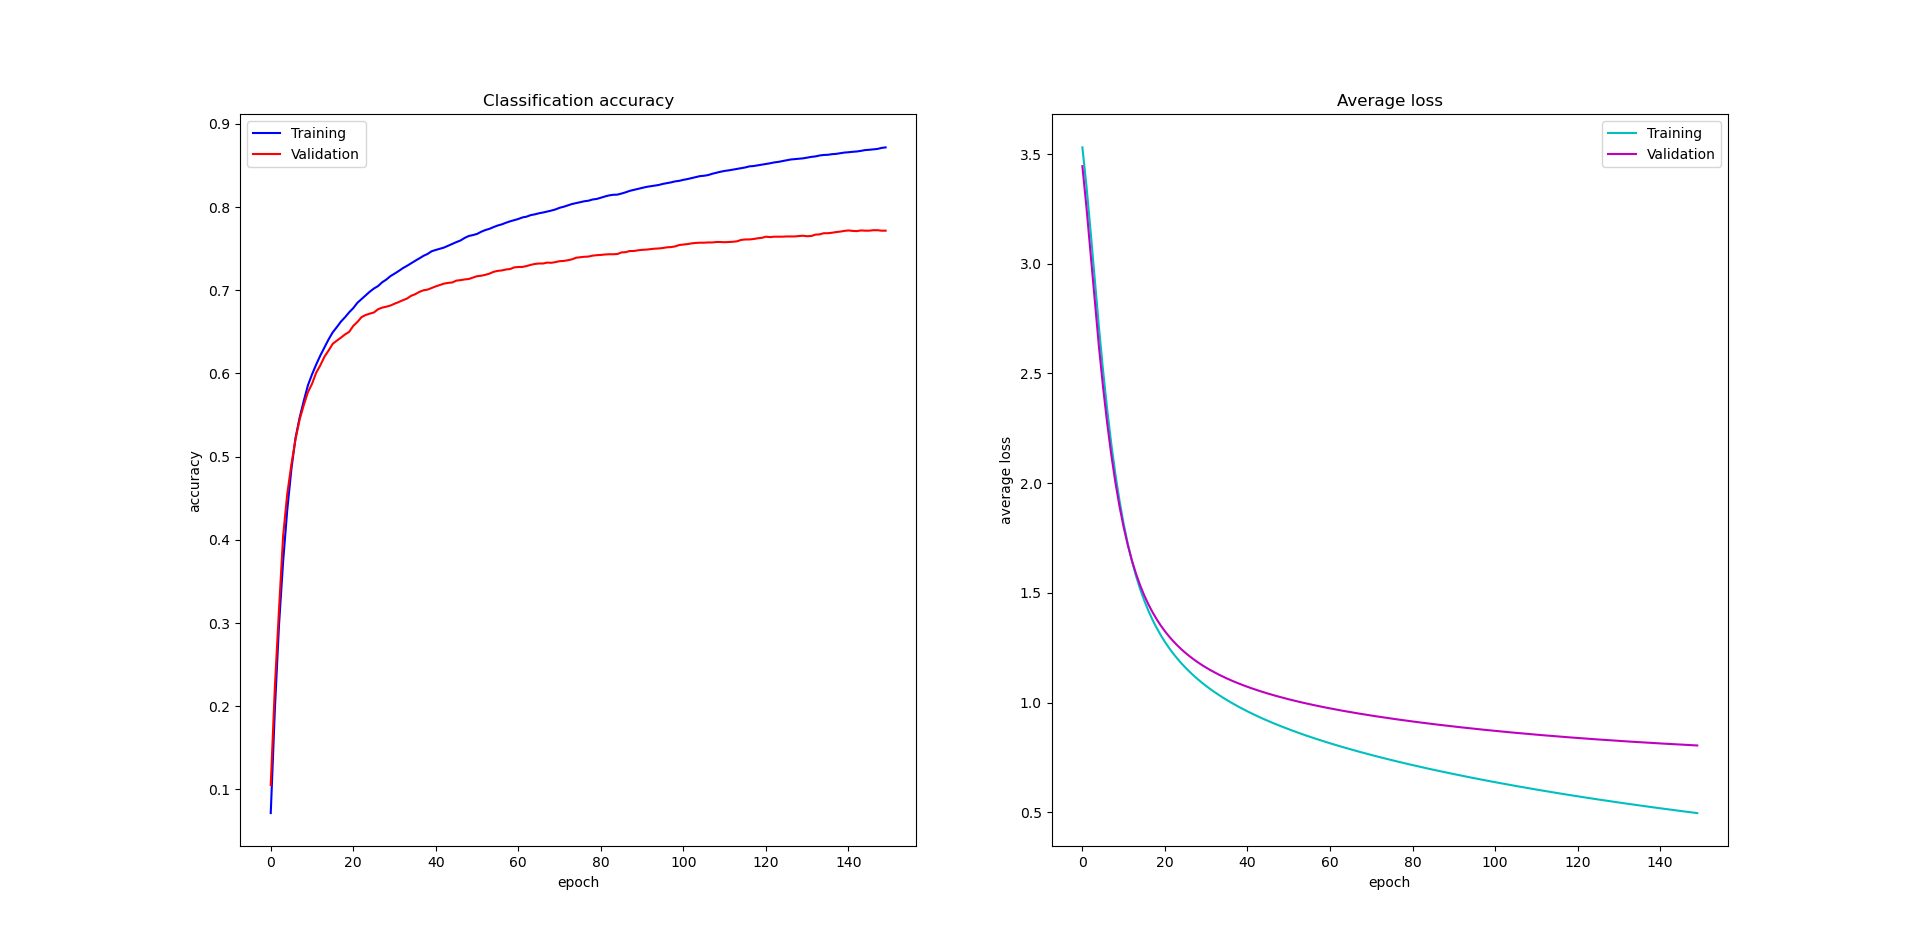
\includegraphics[width=\textwidth]{3,1,2 x0.1 graph.png}
            \caption{Best learning rate}
        \end{subfigure}
        \begin{subfigure}[b]{0.49\textwidth}
            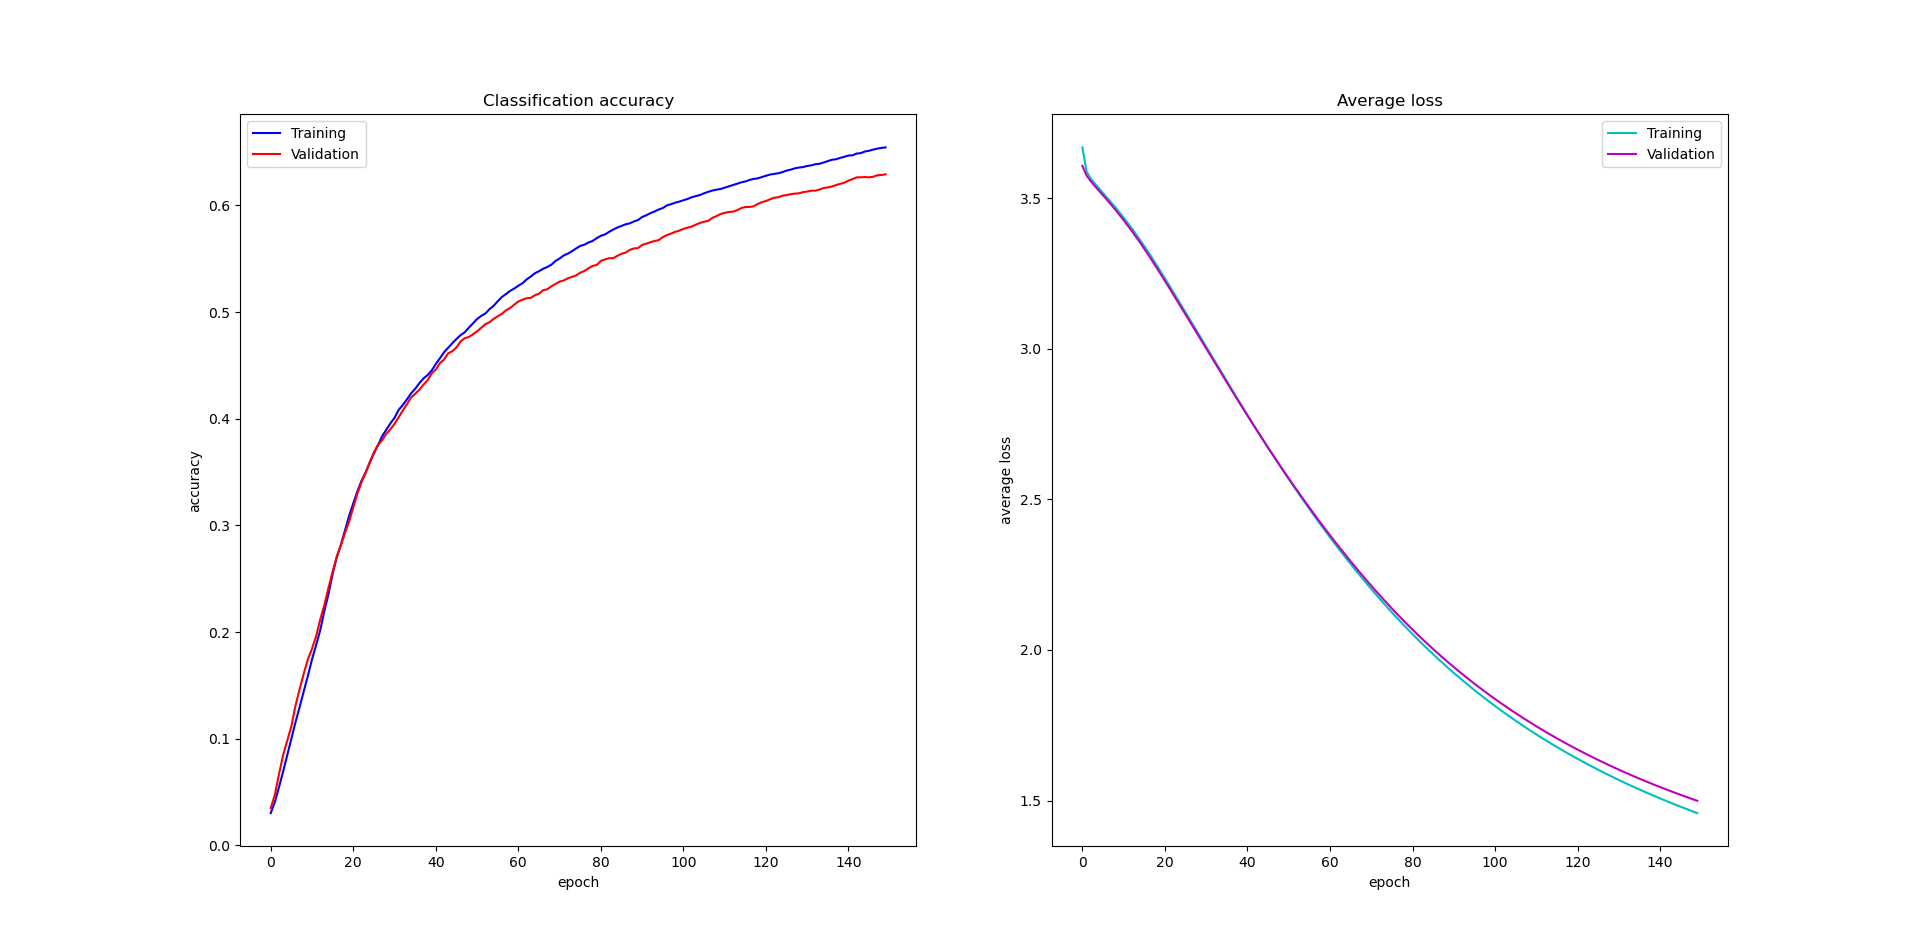
\includegraphics[width=\textwidth]{3,1,2 x0.01 graph.png}
            \caption{$\times1/10$ learning rate}
        \end{subfigure}
        \begin{subfigure}[b]{0.49\textwidth}
        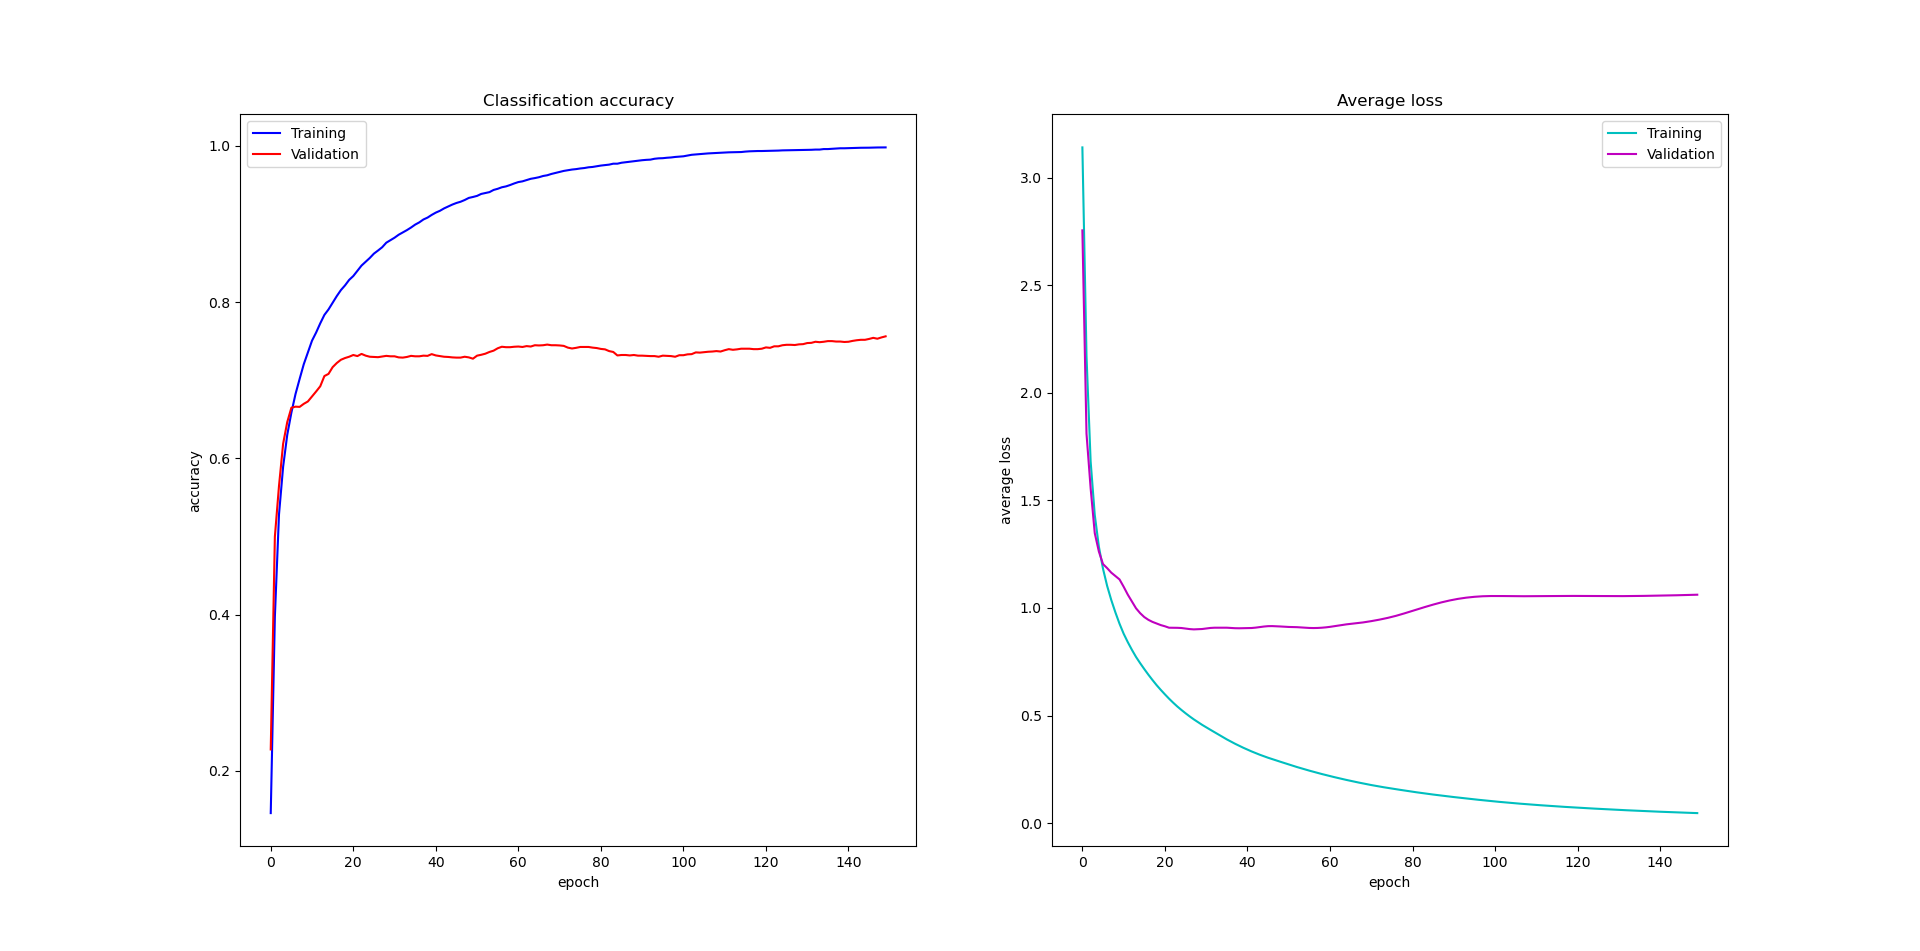
\includegraphics[width=\textwidth]{3,1,2 x1 graph.png}
            \caption{$\times10$ learning rate}
        \end{subfigure}
        \caption{Loss and accuracy curves for three learning rate settings.}
        \label{q312}
    \end{figure}

    Obviously, deviation from most optimal learning rate will decrease accuracy. 
    \medskip

    For a smaller learning rate, gradient descent step size is reduced, leading to slower convergence.
    \medskip

    For a larger learning rate, gradient descent doesn't happen significantly faster, but may cause the loss to increase and fluctuate due to errors induced by large gradient steps (in a similar fashion as the erratic behaviour of large step size in Euler method). Simply said, it is easier to overshoot a local minima with a large step size.
    \medskip
    
    For the best model, \\
    Training Accuracy:  0.8717592592592597 \\
    Validation accuracy:  0.7716666666666666 \\
    Test Accuracy:  0.7844444444444445 

    \subsubsection*{Q3.1.3}
    \begin{figure}[H]
        \centering
        \begin{subfigure}[b]{0.49\textwidth}
            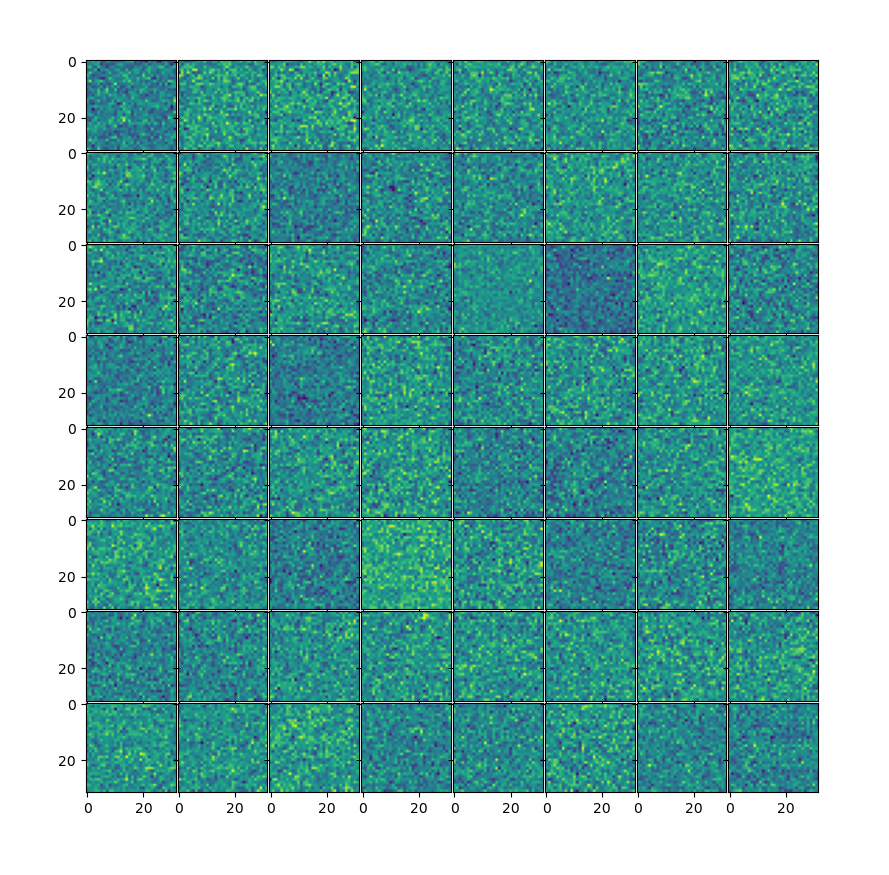
\includegraphics[width=\textwidth]{3,1,3 random weights copy.png}
            \caption{Random weights}
        \end{subfigure}
        \begin{subfigure}[b]{0.49\textwidth}
        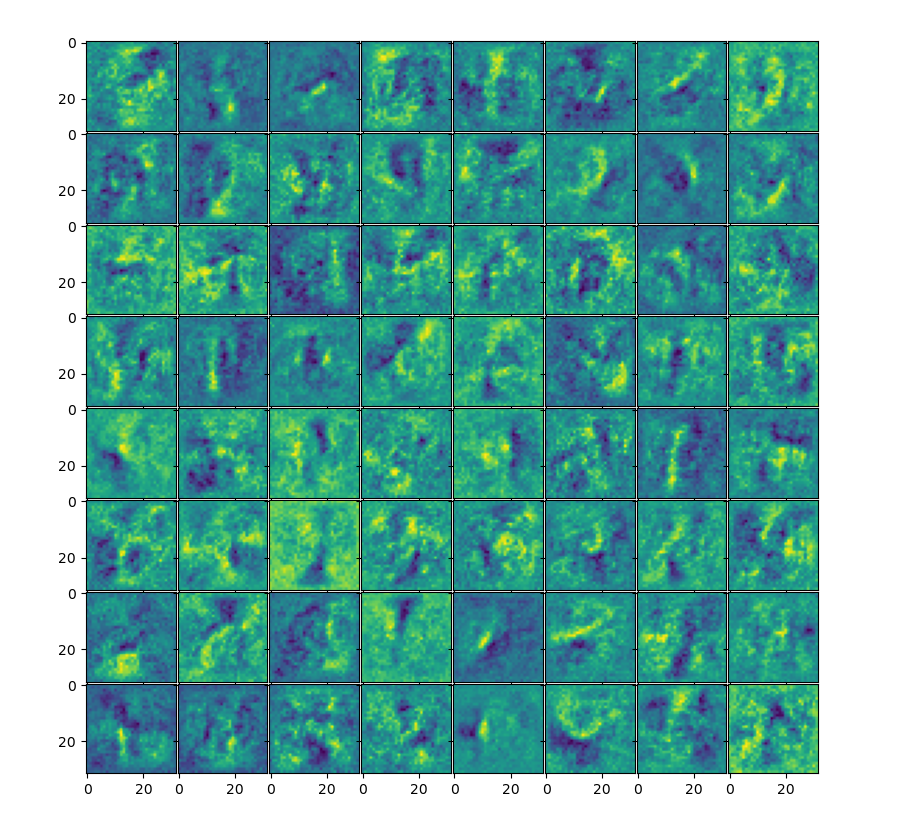
\includegraphics[width=\textwidth]{3,1,3 trained weights copy.png}
            \caption{Trained weights}
        \end{subfigure}
        \caption{Visualized first layer weights of our best model.}
        \label{q313}
    \end{figure}

    Figure \ref{q313} shows the Visualized first layer weights.
    \medskip

    There is no observable pattern in the initial weights, but there are large bright and dark patches in the trained weights. This may signify that the network classifies the characters by seeing if different regions in an image are filled in.
    \medskip

    There are also layers with random weights. These random weights probably failed to train, and their contribution to the final output (i.e. weight to the output layer) is probably small.

    \subsubsection*{Q3.1.4}

    \imgl{3,1,2 x0.1 confusion.png}{Confusion matrix of our best model.}{q314}

    Figure \ref{q314} shows the confusion matrix. The pairs the are most easily confused in this specific network are [0, O], [S, 5], [2, Z], [W, U]. These pairs are structurally similar, and only differ in whether they have sharp corners or not (and corners often become rounded in handwriting) and hence are difficult to differentiate. These letter are usually confused by humans too, but are usually correctable by understanding the context in which the letter is used. However, it would be difficult for the network to differentiate between them.

    \section{Extract Text from Images}
        
    \subsection*{Q4.1}

    Assumptions:
    \begin{enumerate}
        \item Individual characters are clearly written apart and are not connected together by lazy strokes/compact writing. (miss valid letters)
        \item The whole image contains only the piece of paper that the alphabet is written on, and does not include other objects such as the tabletop, cups, pens, etc. All dark pixels detected will be text and not other stuff. (respond to non-letters)
    \end{enumerate}

    Refer to Figure \ref{q41} for the images in which the detection might fail.

    \begin{figure}[H]
        \centering
        \begin{subfigure}[b]{0.49\textwidth}
            \centering
            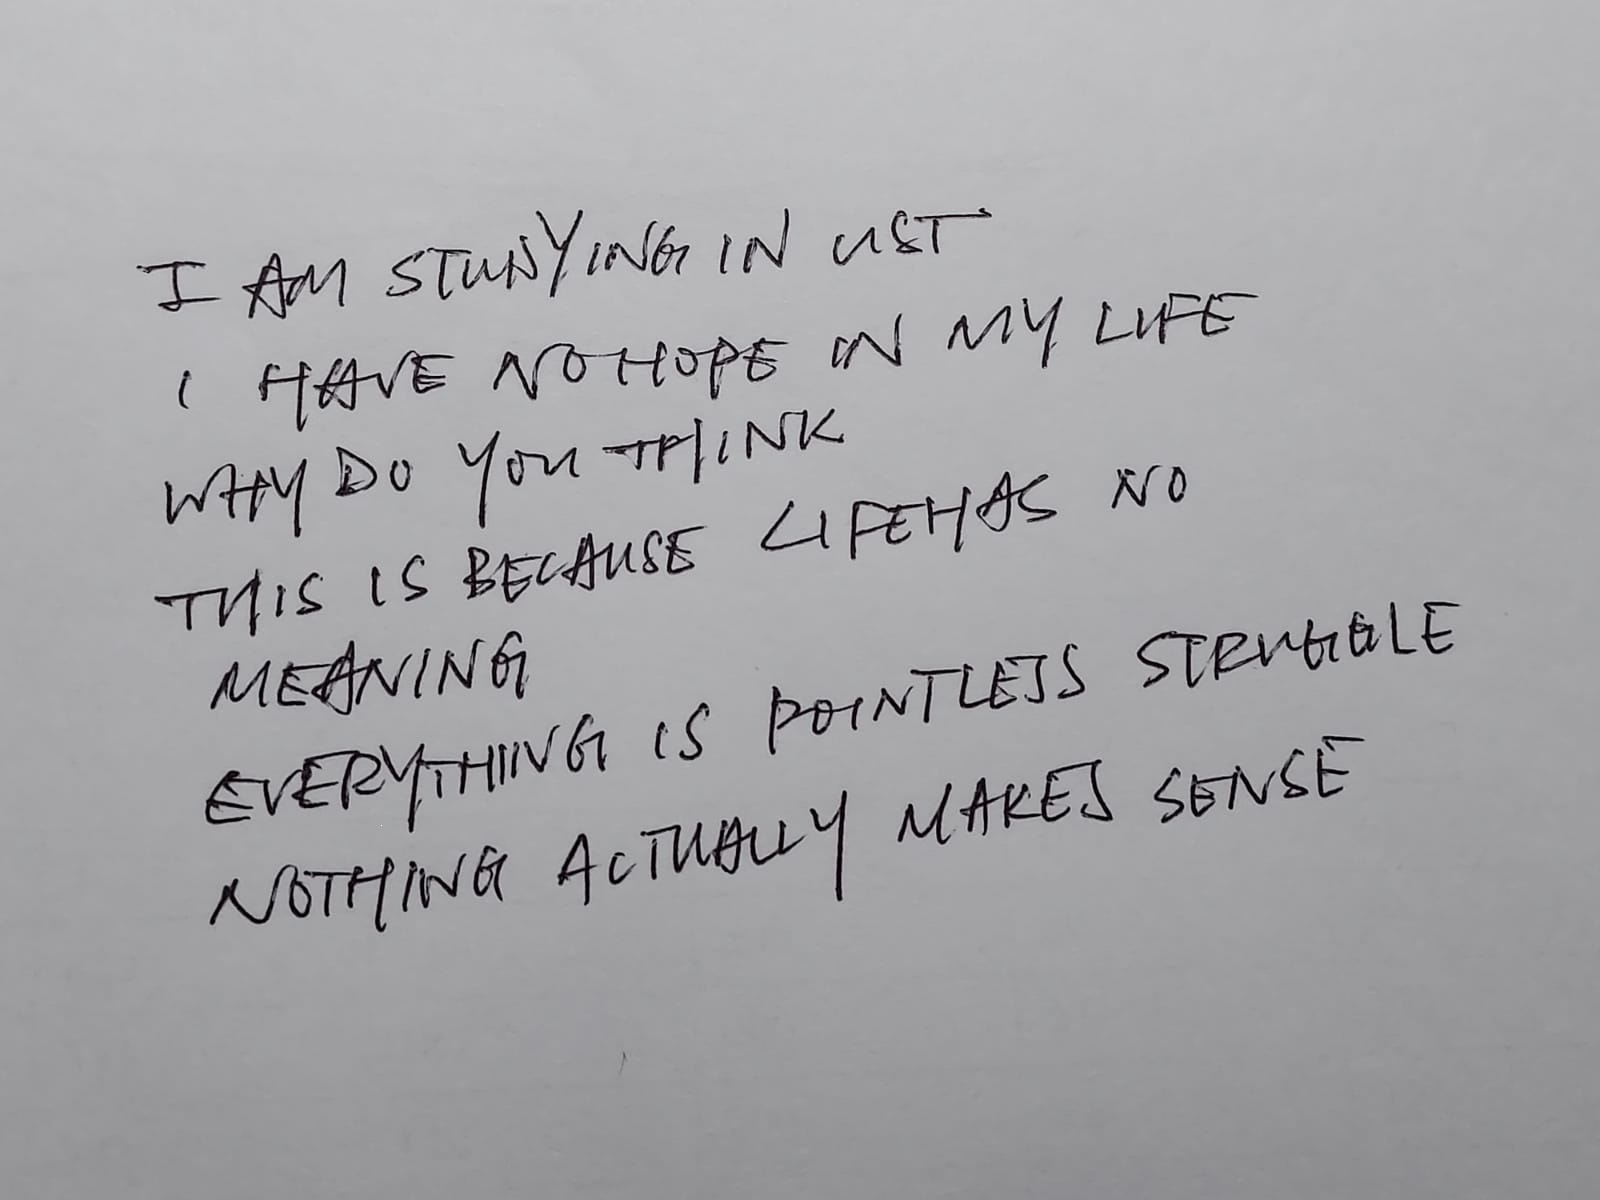
\includegraphics[height=0.3\textheight,width=\textwidth,keepaspectratio=true]{4,1 img2.jpeg}
            \caption{Connected letters}
        \end{subfigure}
        \begin{subfigure}[b]{0.49\textwidth}
            \centering
            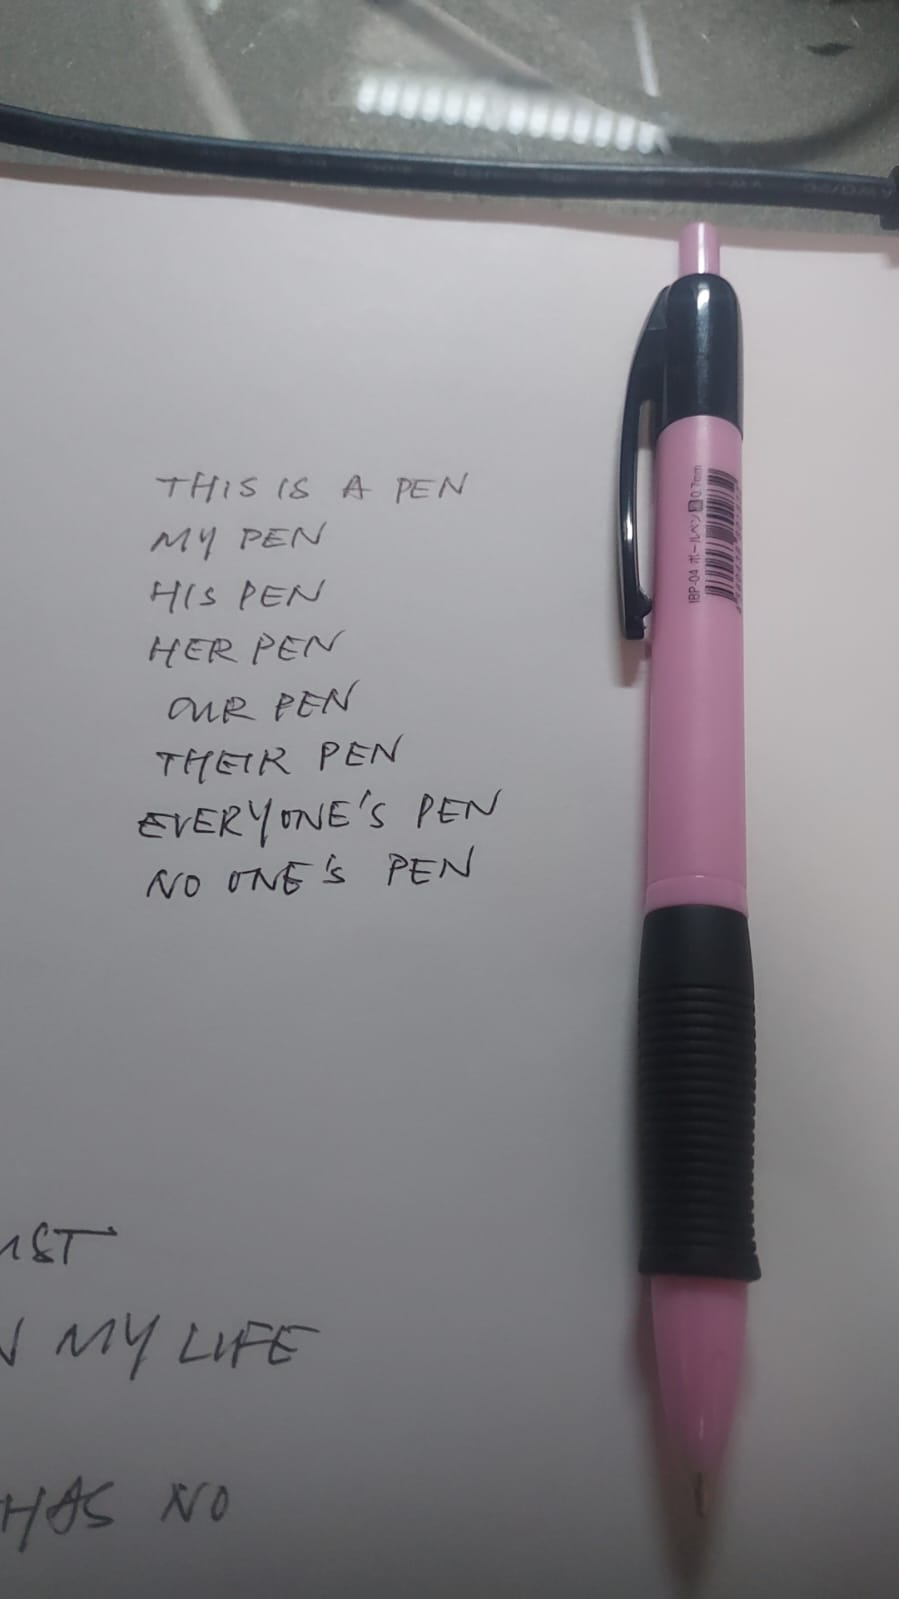
\includegraphics[height=0.3\textheight,width=\textwidth,keepaspectratio=true]{4,1 img1.jpeg}
            \caption{Non-letter objects}
        \end{subfigure}
        \caption{Example images where detection will fail.}
        \label{q41}
    \end{figure}
    
    \subsection*{Q4.3}

    See Figure \ref{q43}.
    
    \begin{figure}[H]
        \centering
        \begin{subfigure}[b]{0.49\textwidth}
            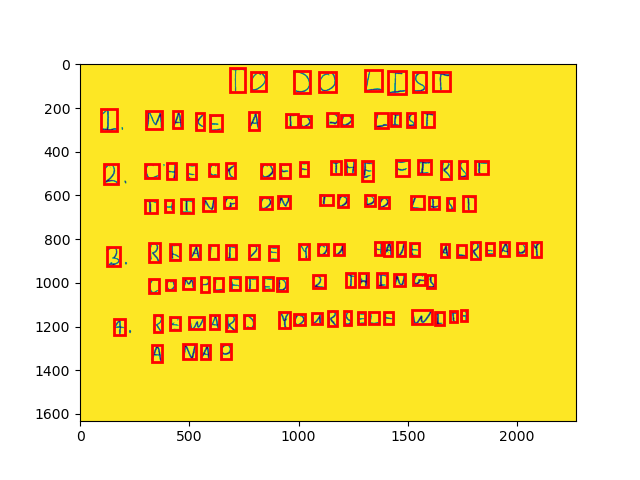
\includegraphics[width=\textwidth]{4,2 img1.png}
        \end{subfigure}
        \begin{subfigure}[b]{0.49\textwidth}
            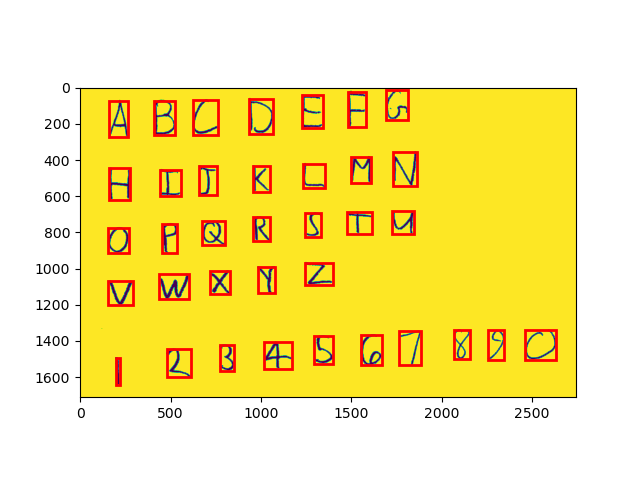
\includegraphics[width=\textwidth]{4,2 img2.png}
        \end{subfigure}
        \begin{subfigure}[b]{0.49\textwidth}
            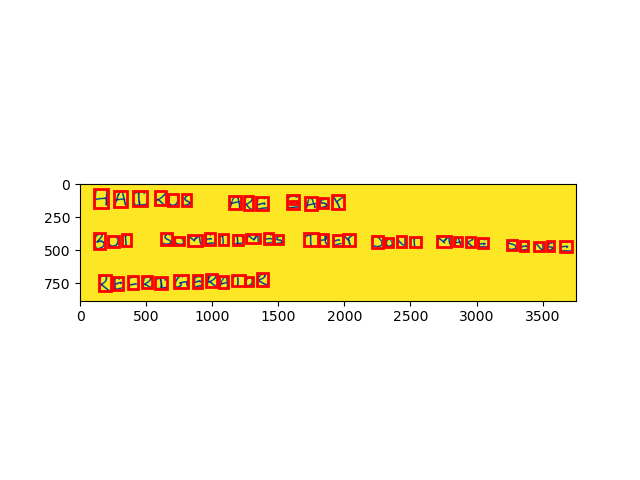
\includegraphics[width=\textwidth]{4,2 img3.png}
        \end{subfigure}
        \begin{subfigure}[b]{0.49\textwidth}
            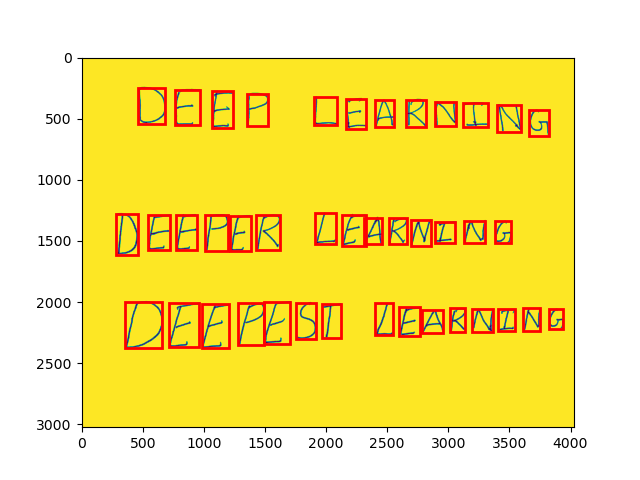
\includegraphics[width=\textwidth]{4,2 img4.png}
        \end{subfigure}
        \caption{Located bounding boxes of letters in each sample image.}
        \label{q43}
    \end{figure}

    \subsection*{Q4.4}
    \bgroup
    \begin{tabular}{||c||c|c||}
        \hline\hline
        & Extracted text & Ground Truth \\
        \hline\hline 
        1 &
\begin{minipage}{0.4\textwidth}\begin{verbatim}

TQDQLIST
IHAK6ATDDGLIST
2LHFCKDFFTHEFIRST
THINGQNTQDQLIST
3RFALIZEY0UHAVBALR6ADT
GQMPLFTLD2THINGS
9RGWARDYQWR5BLFWITB
ANAP

\end{verbatim}\end{minipage}
        &
\begin{minipage}{0.4\textwidth}\begin{verbatim}

TODOLIST
1MAKEATODOLIST
2CHECKOFFTHEFIRST
THINGONTODOLIST
3REALIZEYOUHAVEALREADY
COMPLETED2THINGS
4REWARDYOURSELFWITH
ANAP

\end{verbatim}\end{minipage} \\
\hline
2 &
\begin{minipage}{0.4\textwidth}\begin{verbatim}

ABLDBFG
HIIKLMN
QPQRSTW
VWXTZ
1Z3GSG789Q

\end{verbatim}\end{minipage}
        &
\begin{minipage}{0.4\textwidth}\begin{verbatim}

ABCDEFG
HIJKLMN
OPQRSTU
VWXYZ
1234567890

\end{verbatim}\end{minipage} \\
\hline
3 &
\begin{minipage}{0.4\textwidth}\begin{verbatim}

HAIKUSARGHMAGT
BUTSQMBTIMBGTRETDDNTMAKGBHMQE
RBGRIGBRATQR

\end{verbatim}\end{minipage}
        &
\begin{minipage}{0.4\textwidth}\begin{verbatim}

HAIKUSAREEASY
BUTSOMETIMESTHEYDONTMAKESENSE
REFRIGERATOR

\end{verbatim}\end{minipage} \\
\hline
4 &
\begin{minipage}{0.4\textwidth}\begin{verbatim}

DEBPLEARMING
DBBPERLEARHING
DEEPESPLEARNING

\end{verbatim}\end{minipage}
        &
\begin{minipage}{0.4\textwidth}\begin{verbatim}

DEEPLEARNING
DEEPERLEARNING
DEEPESTLEARNING

\end{verbatim}\end{minipage} \\
    \hline\hline
    \end{tabular}

    \section{Image Compression with Autoencoders}
    \subsection*{Q5.2}
    See Figure \ref{q52} for the curve.
    \medskip

    \imgl{5,2 loss curve.png}{Loss and accuracy curve for autoencoder training.}{q52}

    It can be observed that the training loss curve decreases rapidly at the start, but the decrease quickly dies down at around 8 epochs. After that the loss curve decreases very slowly. 

    \subsection*{Q5.3}
    
    \subsubsection*{Q5.3.1}

    Refer to Figure \ref{q531} for the images.
    \medskip
    
    \begin{figure}[H]
        \centering
        \begin{subfigure}[b]{0.19\textwidth}
            \adjincludegraphics[width=\textwidth,trim={{.3\width} 0 {.3\width} 0},clip]{5,3,1 img0.png}
        \end{subfigure}
        \begin{subfigure}[b]{0.19\textwidth}
            \adjincludegraphics[width=\textwidth,trim={{.3\width} 0 {.3\width} 0},clip]{5,3,1 img1.png}
        \end{subfigure}
        \begin{subfigure}[b]{0.19\textwidth}
            \adjincludegraphics[width=\textwidth,trim={{.3\width} 0 {.3\width} 0},clip]{5,3,1 img2.png}
        \end{subfigure}
        \begin{subfigure}[b]{0.19\textwidth}
            \adjincludegraphics[width=\textwidth,trim={{.3\width} 0 {.3\width} 0},clip]{5,3,1 img3.png}
        \end{subfigure}
        \begin{subfigure}[b]{0.19\textwidth}
            \adjincludegraphics[width=\textwidth,trim={{.3\width} 0 {.3\width} 0},clip]{5,3,1 img4.png}
        \end{subfigure}
        \begin{subfigure}[b]{0.19\textwidth}
            \adjincludegraphics[width=\textwidth,trim={{.3\width} 0 {.3\width} 0},clip]{5,3,1 img5.png}
        \end{subfigure}
        \begin{subfigure}[b]{0.19\textwidth}
            \adjincludegraphics[width=\textwidth,trim={{.3\width} 0 {.3\width} 0},clip]{5,3,1 img6.png}
        \end{subfigure}
        \begin{subfigure}[b]{0.19\textwidth}
            \adjincludegraphics[width=\textwidth,trim={{.3\width} 0 {.3\width} 0},clip]{5,3,1 img7.png}
        \end{subfigure}
        \begin{subfigure}[b]{0.19\textwidth}
            \adjincludegraphics[width=\textwidth,trim={{.3\width} 0 {.3\width} 0},clip]{5,3,1 img8.png}
        \end{subfigure}
        \begin{subfigure}[b]{0.19\textwidth}
            \adjincludegraphics[width=\textwidth,trim={{.3\width} 0 {.3\width} 0},clip]{5,3,1 img9.png}
        \end{subfigure}
        \caption{Reconstruction of validation images using the autoencoder.}
        \label{q531}
    \end{figure}

    Compared to the original image, the autoencoded images are blurry, the colors are more spreaded and diffuse, and often the letters are slightly deformed or show extra lines (e.g. the first image of R has extra lines that look like a D in the background.)

    \subsubsection*{Q5.3.2}

    The PSNR is 15.608972404223165.

    \section{Compare against PCA}
    \subsection*{Q6.1}

    The size of the projection matrix is $32\times1024$, and its rank is $32$.

    \subsection*{Q6.2}

    Refer to Figure \ref{q62} for the images.

    \medskip
    
    \begin{figure}[H]
        \centering
        \begin{subfigure}[b]{0.19\textwidth}
            \adjincludegraphics[width=\textwidth,trim={{.3\width} 0 {.3\width} 0},clip]{6,2 img0.png}
        \end{subfigure}
        \begin{subfigure}[b]{0.19\textwidth}
            \adjincludegraphics[width=\textwidth,trim={{.3\width} 0 {.3\width} 0},clip]{6,2 img1.png}
        \end{subfigure}
        \begin{subfigure}[b]{0.19\textwidth}
            \adjincludegraphics[width=\textwidth,trim={{.3\width} 0 {.3\width} 0},clip]{6,2 img2.png}
        \end{subfigure}
        \begin{subfigure}[b]{0.19\textwidth}
            \adjincludegraphics[width=\textwidth,trim={{.3\width} 0 {.3\width} 0},clip]{6,2 img3.png}
        \end{subfigure}
        \begin{subfigure}[b]{0.19\textwidth}
            \adjincludegraphics[width=\textwidth,trim={{.3\width} 0 {.3\width} 0},clip]{6,2 img4.png}
        \end{subfigure}
        \begin{subfigure}[b]{0.19\textwidth}
            \adjincludegraphics[width=\textwidth,trim={{.3\width} 0 {.3\width} 0},clip]{6,2 img5.png}
        \end{subfigure}
        \begin{subfigure}[b]{0.19\textwidth}
            \adjincludegraphics[width=\textwidth,trim={{.3\width} 0 {.3\width} 0},clip]{6,2 img6.png}
        \end{subfigure}
        \begin{subfigure}[b]{0.19\textwidth}
            \adjincludegraphics[width=\textwidth,trim={{.3\width} 0 {.3\width} 0},clip]{6,2 img7.png}
        \end{subfigure}
        \begin{subfigure}[b]{0.19\textwidth}
            \adjincludegraphics[width=\textwidth,trim={{.3\width} 0 {.3\width} 0},clip]{6,2 img8.png}
        \end{subfigure}
        \begin{subfigure}[b]{0.19\textwidth}
            \adjincludegraphics[width=\textwidth,trim={{.3\width} 0 {.3\width} 0},clip]{6,2 img9.png}
        \end{subfigure}
        \caption{Reconstruction of validation images using PCA.}
        \label{q62}       
    \end{figure}

    Compared to the original images, the images are also blurry and have artifacts that look like other characters behind them. It also has a different background color/value from the original image. When compared with autoencoders, PCA tends to have more background noise, but retains the original shape of the characters better.

    \subsection*{Q6.3}

    The average PSNR is 16.348422786979377. This is slightly better than the autoencoder. 
    \medskip
    
    PCA is Mathematically optimized to retain the greatest amount of feature using its limited range of learning parameters/within its model (a GLOBAL minimum of MSE, its also mentioned in the question that PCA is the "best low-rank approximation"). However, autoencoders are neural networks, which uses only gradient descent and may only be able to reach LOCAL minimas. (Under limited training epochs the solution may not even be optimal!) Therefore, PCA is more robust.

    \subsection*{Q6.4}

    Number of learned parameters for the autoencoder $=1024\times32+32+32^2+32+32^2+32+32\times1024+1024=68704$ (weights and biases), while that for the PCA model is simply $1024\times32=32768$. The reason for the different in performance is explained in Q6.3, with the added note that PCA, even with less parameters, learn better than the autoencoder because of its ability to achieve deterministic global minima of MSE.
    \medskip
    
    Out of curiousity, I ran PCA with 64 dimensions which will have similar learned parameters as the autoencoder, and the PSNR score is 19.00511850049286. We see that under the same number of parameters, PCA outperforms autoencoders by a large margin.

    \section{PyTorch}
    \subsection*{Q7.1}
    \subsubsection*{Q7.1.1}
    The network is implemented in \verb|run_q71.py|.\\
    Training Accuracy:  0.8758333333333339\\
    Validation accuracy:  0.7766666666666666

    \img{7,1 loss acc graph.png}{Q7.1.1 accuracy and loss curve.}

    \subsubsection*{Q7.1.2}
    The network is implemented in \verb|run_q72.py|.\\
    Training accuracy: 0.9632666666666667\\
    Testing accuracy: 0.9762

    \img{7,2 loss acc graph final.png}{Q7.1.2 accuracy and loss curve. Note the loss and accuracy for each minibatch is also plotted using cyan dots.}

    \subsubsection*{Q7.1.3}
    The network is implemented in \verb|run_q73.py|.\\
    Training accuracy: 0.9747222222222223\\
    Testing accuracy: 0.8905555555555555

    \img{7,3 loss acc graph final.png}{Q7.1.3 accuracy and loss curve.}

    \subsubsection*{Q7.1.4}
    The network is implemented in \verb|run_q74.py|.\\
    Training accuracy: 0.9002836879432624\\
    Testing accuracy: 0.8759574468085106

    \img{7,4 loss acc graph final.png}{Q7.1.4 accuracy and loss curve.}

    \begin{tabular}{||c||c|c||}
        \hline\hline
        & Extracted text & Ground Truth \\
        \hline\hline 
        1 &
\begin{minipage}{0.4\textwidth}\begin{verbatim}

T0DQLI5T
LMAKEATDDQLIST
2CHECKDFETHEFIR5T
THINGQNTQDQLf5T
BREALIZEYQUHAVEALREADT
CQMPLETEDZTHINGS
qREWARDYQUR5ELFWITH
ANAP

\end{verbatim}\end{minipage}
        &
\begin{minipage}{0.4\textwidth}\begin{verbatim}

TODOLIST
1MAKEATODOLIST
2CHECKOFFTHEFIRST
THINGONTODOLIST
3REALIZEYOUHAVEALREADY
COMPLETED2THINGS
4REWARDYOURSELFWITH
ANAP

\end{verbatim}\end{minipage} \\
\hline
2 &
\begin{minipage}{0.4\textwidth}\begin{verbatim}

ABCDEFG
HIJKLMN
QPQRSTU
VWXYZ
L2345678g2

\end{verbatim}\end{minipage}
        &
\begin{minipage}{0.4\textwidth}\begin{verbatim}

ABCDEFG
HIJKLMN
OPQRSTU
VWXYZ
1234567890

\end{verbatim}\end{minipage} \\
\hline
3 &
\begin{minipage}{0.4\textwidth}\begin{verbatim}

HAIKUSAREGMA5Y
BUISQMETIMESTKEYDQNTMAKESEN5E
REFRIGERATQR

\end{verbatim}\end{minipage}
        &
\begin{minipage}{0.4\textwidth}\begin{verbatim}

HAIKUSAREEASY
BUTSOMETIMESTHEYDONTMAKESENSE
REFRIGERATOR

\end{verbatim}\end{minipage} \\
\hline
4 &
\begin{minipage}{0.4\textwidth}\begin{verbatim}

DEEPLEARNING
DEEPERLEAKNING
DEEPE5ILEARNING

\end{verbatim}\end{minipage}
        &
\begin{minipage}{0.4\textwidth}\begin{verbatim}

DEEPLEARNING
DEEPERLEARNING
DEEPESTLEARNING

\end{verbatim}\end{minipage} \\
    \hline\hline
    \end{tabular}

    \subsection*{Q7.2}

    It can be seen that the fine-tuned SqueezeNet outperforms the network trained from scratch.
    \subsubsection*{Fine-tuned SqueezeNet}
    The network is implemented in \verb|run_q7part2_squeeze.py|.\\
    Training Accuracy: 1.0
    Validation Accuracy: 0.9382352941176471

    \img{7part2_1 final.png}{Q7.2 fine-tuned SqueezeNet accuracy and loss curve.}

    \subsubsection*{Trained from scratch}
    The network is implemented in \verb|run_q7part2_scratch.py|.\\
    Training Accuracy: 0.7647058823529411 \\
    Validation Accuracy: 0.7

    \img{7part2_2 final.png}{Q7.2 accuracy and loss curve of CNN trained from scratch.}

    
\end{document} % This is the end of the document